\section{Decomposing the prime function unfold}
\label{ap:matrix-power}
\newcommand{\treeunfold}{\mathrm{unfold}}

Among our prime functions, the less satisfactory one is certainly the unfloding function. In this section, we will decompose it into a collection of functions containing no form of iteration. 



\subsection{New prime functions replacing the unfolding}\label{sec:functions-decomposing-unfolding}

The prime functions which are intended to replace the unfolding function use a new datatype constructor called \emph{shallow terms}. it is defined as follows.  

\paragraph*{Shallow terms.} Let $\rSigma$ and $\rGamma$ be two ranked sets. An element of the shallow terms datatype denoted $\shallowterm \rSigma \rGamma$, is an expression of the form $a\tensorpair{b_1,\dots,b_n}$ where $a$ is an $n$-ary element of $\rSigma$ and $b_1,\dots, b_n$ are elements of $\rGamma$. We draw shallow terms like this:
\mypic{54}
Clearly, a shallow term is just a particular case of terms.

\paragraph*{New prime functions.} Let us present now the prime functions which will replace the unfolding function. Prime functions of Figure~\ref{fig:prime-for-shallow-terms} are some basic functions for the new shallow term datatype. Figure~\ref{fig:additional-distrib-prime} contains some new ditributivity laws and Figure~\ref{fig:additional-prime-for-fold} contains some additional laws for the fold datatype. Prime functions of Figure~\ref{fig:weak-unfolding} are weak versions of the unfolding function, containing no form of iteration. 

\newcommand{\simplefun}[4]{
    \begin{tabular}{cc}
        $\ranked{
        \xymatrix@C=1.5cm{
#2 \ar[r]^-{#1}& #3
        }}$
        \\
        {#4}
    \end{tabular}   
 }

 \newcommand{\reversiblefun}[4]{
    \begin{tabular}{cc}
        $\ranked{
        \xymatrix@C=1.5cm{
#2 \ar@<.5ex>[r]^-{#1}& #3
\ar@<.5ex>[l]
        }}$
        \\
        {#4}
    \end{tabular}   
 }



 \newcommand{\laterfun}[3]{
    \begin{tabular}{cc}
        $\ranked{
        \xymatrix@C=1.5cm{
#1 & #2
        }}$
        \\
#3
    \end{tabular}   
 }
 
\begin{definition}[Derivable function]
    The class of \emph{derivable} functions is the least class which:
    \begin{itemize}
        \item contains all arity-preserving functions with finite domain and  the atomic functions (1)--(11);
        \item is closed under function composition and liftings.
    \end{itemize}
\end{definition}

\begin{enumerate}
\item \textbf{The monad $\tmonad$.}
$$\begin{array}{ll}
  \simplefun
        {\unit_\Sigma}
        {\Sigma}
        {\tmonad \Sigma}
        {
      \includegraphics[page=10,scale=0.4]{pics}}
        & 
        \simplefun
        {\flatt_\Sigma}
        {\tmonad \tmonad \Sigma}
        {\tmonad \Sigma} 
        {\tablepic{73}}
\end{array}$$
\item \textbf{The graded monad $\reduce k$.}
$$\begin{array}{ll}
  \simplefun
        {}
        {\Sigma}
        {\reduce 1 \Sigma^1}
        {} &
        \simplefun
        {}
        {\reduce {k_1} \reduce {k_2} \Sigma}
        {\reduce {k_1 \cdot k_2} \Sigma}
        {$(a/f)/g \mapsto a/(g \circ f)$}
        \end{array}$$
\item \textbf{Associativity functions.}
$$\begin{array}{lll}
\ranked{(\Sigma \otimes \Gamma)\otimes \Delta \to \Sigma \otimes (\Gamma\otimes \Delta)} \quad &\quad \ranked{(\Sigma + \Gamma)+ \Delta \to \Sigma + (\Gamma+ \Delta)}  \quad&\quad \ranked{(\Sigma . \Gamma). \Delta \to \Sigma . (\Gamma . \Delta)}
\end{array}$$
\item \textbf{Distributivity functions}.
$$\begin{array}{ll}
      \simplefun
        {}
        {\reduce k (\Sigma_1 + \Sigma_2)}
        {\reduce k \Sigma_1 + \reduce k \Sigma_2}
        {$(a,i)/f \mapsto ((a/f),i)$}
         & 
        \reversiblefun
        {}
        {(\Sigma_1 + \Sigma_2)\otimes \Gamma}
        {(\Sigma_1 \otimes \Gamma) + (\Sigma_2 \otimes \Gamma)}
        {$\tensorpair{(a,i),b} \mapsto (\tensorpair{a,b},i)$}
        \\ \\
        \reversiblefun
        {}
        {\shallowterm {(\Sigma_1 + \Sigma_2)} \Gamma}
        {(\shallowterm {\Sigma_1} \Gamma) + (\shallowterm {\Sigma_2} \Gamma)}
        {$(a,i)\tensorpair{b_1,\ldots,b_n} \mapsto (a\tensorpair{b_1,\ldots,b_n})$ }
        &
        \reversiblefun
        {}
        {\shallowterm {(\Sigma_1 \otimes \Sigma_2)} \Gamma}
        {(\shallowterm {\Sigma_1} \Gamma) \otimes (\shallowterm {\Sigma_2} \Gamma)}
        {
        \begin{tabular}{c}
            $\tensorpair{a_1,a_2}\tensorpair{b_1,\ldots,b_n} \mapsto$ \\
            $\tensorpair{a_1 \tensorpair{b_1,\ldots,b_{n_1}}, a_2\tensorpair{b_{n_1+1},\ldots,b_n} }$  \\
            where $n_1$ is the arity of $a_1$
            \end{tabular}}
            \\
	\simplefun
        {}
        {\reduce k (\Sigma_1 \otimes \Sigma_2)}
        {\reduce k ((\reduce k {\Sigma_1})\otimes (\reduce k \Sigma_2))}{picture}        
	&
	 \simplefun
        {}
        {(\reduce k \Sigma_1) \otimes (\reduce k {\Sigma_2})}
         {\reduce k (\Sigma_1 \otimes \Sigma_2)}
        {picture}  \\
        
         \simplefun
        {}
        {\shallowterm \Sigma {\reduce k \Gamma}}
         {\reduce k (\shallowterm \Sigma {\Gamma})}
        
&        
\end{array} $$
\item \textbf{Commutativity functions.} 
$$\begin{array}{ll}
\ranked{\Sigma_1 + \Sigma_2 \to \Sigma_2 + \Sigma_1} \qquad & \qquad  \ranked{\Sigma_1 \otimes \Sigma_2 \to \Sigma_2 \otimes \Sigma_1}
\end{array}
$$
\item \textbf{Shallow terms.} 
   $$\begin{array}{lll}
   \reversiblefun
        {}
        {\rSigma}
        {\shallowterm 1 {\Sigma} }
        {picture}
        &
      \reversiblefun
        {}
        {\rSigma}
        {\shallowterm {\Sigma} 1}
        {picture}
        &
        \reversiblefun
        {\composeterm}
        {1 + \shallowterm \Sigma {\tmonad \Sigma} }
        { \tmonad \Sigma}
        {
        \begin{tabular}{c}
            Every term is either just a port,\\ or has a root and child subterms.    
        \end{tabular}    
        } 
\end{array} $$     
\item \textbf{The error type $\bot$.} Some error raising mechanisms.
$$\begin{array}{llll}
\ranked{\Sigma \to \bot} \quad&\quad \ranked{\tmonad(\Sigma+\bot)\to \tmonad\Sigma+\bot} \quad&\quad \ranked{\reduce k (\Sigma+\bot)\to \reduce k\Sigma+\bot}\quad&\quad  \ranked{(\Sigma+\bot)\otimes \Gamma\to \Sigma\otimes \Gamma+\bot}
\end{array}$$     
\item \textbf{Injections.}
$$\begin{array}{llll}
\ranked{\Sigma \to \Sigma+\Sigma} \quad &\quad \ranked{\Sigma \to \reduce k \Sigma^k}  \quad & \quad \ranked{\reduce k \Sigma \to \reduce {k+l}\Sigma} \quad & \quad 
\ranked{\Sigma^n\to  \shallowterm n \Sigma}
\end{array}$$
\item \textbf{Projections.}
$$\begin{array}{llll}
\ranked{\Sigma+\Sigma\to \Sigma} \quad &\quad \ranked{\Sigma\otimes \Sigma \to \reduce 1 \Sigma} \quad & \quad \ranked{\reduce {k+1} \Sigma \to \reduce {k}\Sigma+\bot} \quad & \quad 
\ranked{\shallowterm n \Sigma \to \Sigma^n} 
\end{array}$$
\item \textbf{Factorisations.} Same as before.
\item \textbf{Pre-order.} Same as before.
\item \textbf{Unfolding.} In addition to the shallow unfold, 
 we consider also \emph{the unfolding of external twists}. This function, which is of type 
\begin{align*}
\ranked{\tmonad \mati k \Sigma \to \reduce k \tmonad \mati k \Sigma}
\end{align*}
"untwists" the external twists  as illustrated by the following figure where the external twists have been colored in red. 
\begin{center}
\includegraphics[scale=.4]{external-unfold.pdf}
\end{center}
\end{enumerate}




The main result of this section is that the unfolding can be replaced by the more atomic functions of Figures~\ref{fig:prime-for-shallow-terms}, \ref{fig:additional-distrib-prime}, \ref{fig:additional-prime-for-fold} and ~\ref{fig:weak-unfolding}, in  presence of the other prime functions presented in Section~\ref{sec:derivable-functions}, as stated in the following theorem
 
\begin{theorem}\label{thm:decompose-unfolding}
The unfolding function can be derived using the functions of Figures~\ref{fig:prime-for-shallow-terms}, \ref{fig:additional-distrib-prime}, \ref{fig:additional-prime-for-fold}, ~\ref{fig:weak-unfolding}, and the prime functions of Section~\ref{sec:derivable-functions}.
\end{theorem}

%\subsection{Decomposing the unfolding function}\label{sec:proof-decompose-unfold}


Our proof strategy is to show that term unfolding can be derived for certain homogeneous (see below) monotone inputs, and then to show that every input can be decomposed into simpler inputs in a homogeneous way. The notion of homogeneous inputs, and the result about  decomposing of arbitrary inputs into homogeneous inputs, are presented in Section~\ref{sec:factfor}. Next, in Section~\ref{sec:homo-unfold}, we show how term unfolding can be done for homogeneous inputs. Finally, in Section~\ref{sec:monotone-unfold-proof} we prove Theorem~\ref{thm:decompose-unfolding} by combining  the results of Sections~\ref{sec:factfor} and~\ref{sec:homo-unfold}.

\subsection{Factorisation forests}
\label{sec:factfor}
This section is devoted to stating and proving a tree version of the Factorisation Forest Theorem of Imre Simon.  Our result differs from the original Factorisation Forest Theorem in the following ways: (a) we consider trees instead of strings; (b) we use aperiodic finite monoids instead of arbitrary finite monoids; and (c) the factorisation in the conclusion of the theorem can be computed by a derivable function.  A tree generalisation of the Factorisation Forest Theorem was already proved by Colcombet~\cite[Theorem 1 and Section 3.3]{colcombetCombinatorialTheoremTrees2007}, but Colcombet's result is proved for monadic second-order logic, and therefore it does not satisfy condition (c). 



\paragraph{Factorisation forests} The idea behind factorisation forests is to split a term into a nested factorisation, which is a term of terms of terms, and so on up to a certain depth.  
Define a \emph{nested factorisation} of depth $k \in \set{1,2,\ldots}$ over alphabet $\rSigma$ to be an element of $\tmonadn k \rSigma$ which is defined by
\begin{align*}
\tmonadn 0 \rSigma = \rSigma  \quad \text{and} \quad \tmonadn {k+1}\rSigma = \tmonad \tmonadn k \rSigma.
\end{align*}
Nested factorisations can be flattened to terms by using an  operation $\flatn k : \tmonadn k \rSigma \rto \tmonad \rSigma $ defined by 
\begin{align*}
     \flatn 1 = \text{\ranked{identity}} \quad \text{and} \quad  \flatn {k+1} \eqdef \flatt  \circ \tmonad \redpar { \flatn k}.
\end{align*}
An equivalent definition of $\flatn {k+1}$ would be $\flatn k \circ \tmonadn {k-1} \flatt$, the equivalence of these definitions corresponds to the fact that $\tmonad$ is a monad.


\paragraph{Branches and subbranches}
Define a \emph{branch} in a ranked set to be an element  of the ranked set together with a distinguished port. 
We draw branches like  this:
\mypic{82}
For a term, we classify its edges as internal (linking a non-port node with a non-port child) and external (linking a non-port node with a child port). Each edge in a term $t \in \tmonad \rSigma$ corresponds to a branch over $\rSigma$, namely the branch which leads to the edge. Any branch obtained this way is called a \emph{subbranch} of $t$. Here is a picture of subbranches in the case of a term of terms:
\mypic{80} 

\newcommand{\hb}[2]{#2^{(#1)}}
Branches in  terms  form a monoid. Using the monoid structure of branches in terms, we can extend any function  $h : \branches \rSigma \to M$, with $M$ a monoid, to a  monoid homomorphism
\begin{align*}
\hb n h : \branches \tmonadn n \rSigma \to M
\end{align*}
which maps a branch of a term to the product -- in the monoid $M$ -- of all of its subbranches (after flattening).  A more formal definition is that $\hb 0 h$ is the same as $h$, while  $\hb {n+1} h$  is the unique monoid homomorphism  which makes the following diagram commute
\begin{align*}
\xymatrix{
    \branches \tmonadn n \rSigma \ar[dr]^{\hb n h} \ar[d]_{\branches \unit}\\
    \ar[r]_{\hb {n+1}  h}\branches \tmonadn {n+1} \rSigma & M
}
\end{align*}


The idea behind factorisation forests, as expressed in Definition~\ref{def:hom-for} below, is to factorise a term into a term of terms of terms (etc.) so that the depth of nesting is bounded, and at each level all branches behave regularly with respect to some monoid homomorphism. 

\begin{definition}[Homogeneous factorisations]\label{def:hom-for}
    Let $h : \branches \rSigma \to M$ be a function into a monoid $M$. 
    \begin{itemize}
\item     We say that a factorisation $t \in \tmonad \tmonad \rSigma$ is \emph{homogeneous with respect to $h$} if it either:
\begin{enumerate}
    \item \label{it:factfor-shallow} it is a shallow term (which means that all internal edges originate from the root); or 
    \item \label{it:factfor-allsame} all internal subbranches of $t$ have the same value under $\hb 1 h$; or
    \item \label{it:factfor-ab} if $a,b \in M$ appear as values -- under $\hb 1 h$ -- of internal branches in $t$, then $ab=a$. 
\end{enumerate}
\item We say that a nested factorisation  $t \in \tmonadn n \rSigma$ is \emph{hereditarily homogeneous with respect to $h$} if either $n=1$ and $t$ is the unit of a letter, or $n \ge 2$ and both:
\begin{enumerate}
    \item  it is homogeneous with respect to $\hb {n-1} h$; and 
    \item every node has a label in $\tmonadn {n-1} \rSigma$ that is hereditarily homogeneous with respect to $h$.
\end{enumerate}
    \end{itemize}
\end{definition}


Recall that a finite monoid is aperiodic if it has only trivial subgroups. An equivalent definition is that every element $m$ of the monoid satisfies 
\begin{align*}
  \exists n \in \set{1,2,\ldots}\   m^n = m^{n+1}.
\end{align*} 
A famous theorem of Sch\"utzenberger, McNaughton and Papert, see~\cite[Theorem VI.1.1]{straubingFiniteAutomataFormal1994} says that the languages  of words recognised by homomorphisms into finite aperiodic monoids are exactly  those that can be defined in first-order logic. This is the reason why  we consider aperiodic monoids.

\begin{example}\label{ex:partial-monoton-functions}
   Let $k \in \set{1,\ldots}$ and  consider the monoid of partial functions 
    \begin{align*}
    \set{1,\ldots,k} \to \set{1,\ldots,k}.
    \end{align*}
    This monoid is not aperiodic, because it contains the  group of all permutations of $\set{1,\ldots,k}$. Consider now the restriction of this monoid to partial functions which are monotone (this is a monoid, because such functions are closed under composition). This monoid is aperiodic, because if $f$ is a partial function, then for  every $i \in \set{1,2,\ldots,k}$ the sequence
    \begin{align*}
    f^1(k),f^2(k),f^3(k),\ldots
    \end{align*}
    reaches a fixpoint (or becomes undefined) in at most $k$ steps.
\end{example}
We are now ready to state our version of the Factorisation Forest Theorem. 
\begin{theorem}[Factorisation Forest Theorem]\label{thm:factfor}
    Let $\rSigma$ be a  ranked set and let $h : \branches  \rSigma \to M$ be a function into a finite aperiodic monoid $M$. There is some $n \in \set{1,2,\ldots}$ and a  function
    \begin{align*}
        \ranked {f : \tmonad \rSigma \to \tmonad^n \rSigma}  
    \end{align*}
such that $\flatn n \circ \ranked f$ is the identity on $\tmonad \rSigma$, and  all outputs of  $\ranked f$ are hereditarily homogeneous with respect to $h$. Furthermore, if $\rSigma$ is finite\footnote{This finiteness assumption could be relaxed by saying that $\rSigma$ is possibly infinite but the function $h$ is derivable, in the sense that a derivable function can decorate the ports of an element in $\rSigma$ by their values under $M$.} then $\ranked f$ is derivable. 
\end{theorem}



\newcommand{\hint}{\bar h}
\newcommand{\hintplus}{\bar h^+}
\newcommand{\branchesplus}{\mathsf B^+}


% Later in this section, we also give a sufficient condition which ensures that $\ranked f$ as in the theorem is derivable, by analysing in more detail the proof the theorem. 
In the proof below, the constructions  are designed so that they can be formalised using derivable functions, however we leave the details of  the ``Furthermore'' part to the reader. 

Define a \emph{good set} to be any subset  $\ranked X \subseteq  \tmonad \rSigma$ which admits a function 
\begin{align*}
    \ranked {f : \tmonad \rSigma \to \tmonad^n \rSigma}   \qquad \text{for some $n \in \set{1,2,\ldots}$}
\end{align*}
such that $\flatn n \circ \ranked f$ is the identity on $\tmonad \rSigma$, and    $\ranked f$ restricted to $\ranked X$ produces only hereditarily homogeneous outputs. Our goal is to show that the entire set $\tmonad \rSigma$ is good. To prove this, we use a more refined result, stated below, which has a parameter  that can be used for  induction.  We say that a term $t \in \tmonad \rSigma$ uses $A \subseteq M$ for  internal subbranches if all  internal subbranch have image under $\hb 1 h$ that belongs to $A$. 

\begin{lemma}\label{lem:fact-ind}
    Let $\rSigma$ be a  ranked set and let $h : \branches \tmonad \rSigma \to M$ be a monoid homomorphism into a finite aperiodic monoid $M$. For every $A \subseteq M$, the  terms that use $A$ for inner subbranches  is good.
    \end{lemma}

\newcommand{\subgen}[1]{\langle #1 \rangle}
Theorem~\ref{thm:factfor} follows immediately from the  lemma, by taking $A$ to be the entire monoid. The rest of Section~\ref{sec:factfor} is therefore devoted to proving the lemma. The proof is by induction on  two parameters: (a) the size of $A$; and (b) 
the size of the semigroup $\subgen A \subseteq M$ that is  generated by $A$.
 These parameters are  ordered lexicographically, with the size of the semigroup being more important.

The induction base is when $A$ contains only one element $a$ of the monoid. If a term uses $\set a$ for  internal subbranches, then applying $\tmonad \unit$ leads to a factorisation that is  homogeneous according to item~\ref{it:factfor-allsame} of Definition~\ref{def:hom-for}, which is also hereditarily homogeneous because all nodes are labelled by units. This completes the proof of the induction base.

In the proof of the induction step, we consider two cases.
\begin{itemize}
    \item The first case is  when  every $a \in A$ satisfies 
    \begin{align*}
       \subgen{\set{ b a :  b \in \subgen A}} = \subgen A
  \end{align*}
  This means that every for every $a \in A$, the function $b \mapsto ba$ is a permutation of $\subgen A$. Since the monoid is aperiodic, this permutation must necessarily be the identity.  Therefore, we have $ab=a$ for every $a,b \in \subgen A$. This means that if all a term uses $A$ for  internal subbranches, then applying $\tmonad \unit$  gives a factorisation which is hereditarily homogeneous according to item~\ref{it:factfor-ab} of Definition~\ref{def:hom-for}. 
    \item If the previous item does not hold, then there is some $a \in A$ such that 
    \begin{align*}
         \subgen{\set{ b a :  b \in \subgen A}}
    \end{align*}
    is a proper subsemigroup of $\subgen A$.  Fix some such $a$.  Define a \emph{sensitive edge} in a term  $t \in \tmonad \rSigma$ to be any internal edge where the corresponding subbranch has value $a$ under  $\hb 1 h$. Call an internal edge \emph{post-sensitive} if it is not sensitive, but its parent edge is. Here is picture:
    \mypic{8}
    Define the \emph{split} of a term to be the factorisation which  cuts along post-sensitive  edges, as shown in the following picture:
    \mypic{88}
    We only consider splits for terms which use $A$ for internal subbranches. Roughly speaking,  we will show that all factors in the split are good, and the split itself is good.  Combining these two observations, we will see that all terms 

    We begin by looking at the factors in the split (of a term where $A$ is used for internal subbranches). Here is a picture of such a factor:
    \mypic{89}
        If we follow a  branch in an factor of the split, from root to port, we first  have a sequence of non-sensitive  edges from the original term, followed by a sequence of sensitive edges. Group the non-sensitive edges together, and group the sensitive edges together, resulting in a shallow term from $\shallowterm{\tmonad \rSigma}{\tmonad \rSigma}$, which is illustrated in the following picture:
    \mypic{90}
        In the resulting shallow term,  the root is labelled by a term without sensitive edges (i.e.~it is a term which uses $A - \set a$ for internal subbranches), while the children are labelled by terms where all edges are sensitive (i.e.~they are terms which use $\set a$ for internal subbranches). We can apply the induction in both cases, and combine the resulting nested factorisations using a shallow term, as in item~\ref{it:factfor-shallow} of Definition~\ref{def:hom-for}.

        Having established that the factors of the split are good, we turn to the split itself. By construction, every subbranch of the split is mapped by $\hb 1 h$ to the smaller semigroup 
        \begin{align*}
            \subgen{\set{ b a :  b \in \subgen A}},
       \end{align*}
       We can  view the  split as a term over alphabet $\rGamma = \tmonad \rSigma$.  Since all  internal subbranches of the split are in the smaller subsemigroup, we can apply the induction assumption of the lemma (with $\rGamma$ and $\hb 1 h$), showing that the split is good. More formally, the set 
       \begin{align*}
       \set{\text{split of $t$} : t \in \tmonad  \rGamma \text{ uses $A$ for internal subbranches}}
       \end{align*}
       is good. To show now that original set of terms $t$ that use $A$ for  internal branches is good, we first apply the split, then compute the nested factorisation for the split, and finally we compute the nested factorisations for the factors of the split (the letters from $\rGamma$.). 
\end{itemize}


% We now give a proof sketch of the ``Furthermore'' part in the theorem, which says that if $\rSigma$ is finite, then
% \begin{align*}
%     \ranked {f : \tmonad \rSigma \to \tmonad^k \rSigma}  
% \end{align*}
% in the conclusion of the theorem not only exists, but it is derivable. In the proof sketch, we will appeal to the power of first-order tree relabellings from Section~\ref{sec:fo-translation}. To use tree relabellings, define \emph{pseudo-flattening} to be the  function 
% \begin{align*}
% \ranked{\mathrm{pseudoflat}} : \tmonad \tmonad \rSigma \rto \tmonad\redpar{\rSigma \redplus \redset{\overbrace{\text{open},\text{close}}^{\text{arity 2}}}}
% \end{align*}
% which adds an ``open'' whenever a new factor starts and adds a ``close'' letter whenever a factor ends, as depicted in the following picture:
% \mypic{91}
% Pseudo-flattening can be lifted in a natural way to nested factorisations 
% \begin{align*}
%     \ranked{\mathrm{pseudoflat}_n : \tmonadn {n+1} \rSigma \rto \tmonad \Sigma_n} \qquad \text{where }\ranked{\Sigma_n} \eqdef \redpar{\rSigma \redplus \redset{\overbrace{{\text{open}_i,\text{close}_i }}^{\text{arity 2}: i \in \set{1,\ldots,n}}}}
% \end{align*}
% Call a function $\ranked f$  \emph{pseudo-derivable} if there  is a derivable $\ranked g$ which makes the following diagram commute
%     \begin{align*}
%     \ranked{
%         \xymatrix{
%             \tmonad \rSigma \ar[r]^f \ar[d]_{\mathrm{pseudoflat}}& \tmonadn n \rSigma \ar[d]^{\mathrm{pseudoflat_n}} \\
%             \tmonad \rSigma_1 \ar[r]_g & \tmonad \rSigma_n 
%         }
%     }
%     \end{align*}
    
% \begin{lemma}\label{lem:pseudo-der}
%     A function $\ranked f$ is derivable if and only if it is pseudo-derivable.    
% \end{lemma}
% \begin{proof}
%     (Sketch.) Pseudo-flattening and its nested extensions are  easily seen to be derivable, and the same is true for their (one-sided) inverses.  
% \end{proof}
 
% The advantage of  pseudo-flattening  is that it allows use to work with first-order tree relabellings, which are much easier to work with. By an analysing the proof of Lemma~\ref{lem:fact-ind}, one can show that if $\rSigma$ is finite, then  the function $\ranked f$ is pseudo-derivable. This is because the basic operations in the proof of the lemma, such as ``find the first sensitive edge'' can easily be formalised in first-order logic, which in turn can be turned into derivable functions by virtue of Proposition~\ref{prop:forat}. 

\subsection{Term unfolding for homogeneous inputs}
\label{sec:homo-unfold}



\subsubsection{Term unfolding for $\alpha$-homogeneous inputs}
\label{subsec:alpha-homo-unfold}

For a monotone function 
\begin{align*}
\alpha: \set{1,\ldots,k} \to \set{1,\ldots,k}
\end{align*}
we say that a term $ t \in \tmonad \mati k \rSigma$ is $\alpha$-homogeneous if all internal branches have twist $\alpha$. This section is devoted to proving the following lemma. 

\begin{lemma}\label{lem:homo-twist}
    Let $k \in \set{1,2,\ldots}$ and let $\alpha : \set{1,\ldots,k} \to \set{1,\ldots,k}$ be a monotone function. There is a derivable operation 
    \begin{align*}
        \ranked{f : \tmonad \mati k \rSigma \to \mati k {(\tmonad \Sigma)} }
        \end{align*}      
which coincides with term unfolding for all inputs which are $\alpha$-homogeneous.
\end{lemma}

\begin{proof}
We proceed by induction on $k$. When $k=1$, the unfolding coincides with the basic distributivity function 
\begin{align*}
\ranked{ \tmonad \reduce 1 \Sigma \to {\reduce 1 \tmonad \Sigma}}
\end{align*}
Let us treat the inductive case. For that, we introduce a tool that will be useful to analyze the function $\alpha$. For a function $$\alpha: \set{1,\ldots,k} \to \set{1,\ldots,k}$$ define  \emph{its graph} as the directed graph whose set of vertices is $\set{1,\ldots,k}$, and which contains an edge $i\rightarrow j$ if $\alpha(i)=j$. Note that the out-degree of the nodes is $1.$

\medskip
In the proof of the inductive case, we distinguish two cases. The first one is when the graph of $\alpha$ is not weakly connected. In this case, by monotonicity of $\alpha$, we can find $m\in \set{1,k-1}$ such that $\alpha(\set{1,m})\subseteq\set{1,m}$ and $\alpha(\set{m+1,k})\subseteq\set{m+1,k}$. The idea is then to create two copies of the original tree: in the first one we keep only the first $m$ elements of the tensor product of each node, and in the second one we keep the last $k-m$ copies. Then we unfold these terms by applying the induction hypothesis, and  finally we gather them to obtain the  unfolding of the original term. 

%\smallskip
%To illustrate this case, we consider the following function $\alpha$, whose graph is shown below
%\begin{center}
%\includegraphics[scale=.07]{MyPic27.jpg}
%\end{center}
%The graph of $\alpha$ is not weakly connected: it contains two weakly connected components, $\set{1,2}$ and $\set{3}$.
%Consider the following $\alpha$-homogeneous terms $t$ of $\tmonad \mati k \rSigma$ which will be our running example in the not weakly connected case of the proof. We colored in blue the elements of the first weakly connected part of the graph of $\alpha$ and in green the second part.
%\begin{center}
%\includegraphics[scale=.07]{MyPic28.jpg}
%\end{center}
Let us now implement the ideas we discussed above. We start by unfolding the external twists, using the basic external unfold function. This way, the domain of every external twist  cannot be shared by the two disconnected components of the domain of $\alpha$.
%Our running example becomes like this:
%\begin{center}
%\includegraphics[scale=.07]{MyPic29.jpg}
%\end{center}
Then, we duplicate the input term using the basic function 
\begin{align*}
\ranked{\tmonad \mati k \Sigma\to \reduce 2 (\tmonad \mati k \Sigma\otimes \tmonad \mati k \Sigma)}
\end{align*}
To the first copy, we apply the function  
\begin{align*}
\ranked{f_1:\tmonad \mati k \Sigma \to \mati m {(\tmonad \Sigma)}}
\end{align*}
which keeps only the first $m$ elements of the tensor product, then applies the induction hypothesis to the obtained term.
To the second copy, we apply the function 
\begin{align*}
\ranked{f_2:\tmonad \mati k \Sigma \to \mati {k-m} {(\tmonad \Sigma)}}
\end{align*}
which keeps only the last $k-m$ elements of the tensor product, then applies the induction hypothesis to the obtained term.

%Here is the effect of the functions $f_1$ and $f_2$ on our example
%\begin{center}
%\includegraphics[scale=.15]{MyPic30.jpg}
%\end{center}
 The function $\ranked{f_1}$ can be derived using the tensor projection function, the merge of folds, then reducing the fold and finally invoking the induction hypothesis. 
%\begin{align*}
%\begin{prooftree}
%\Hypo{\overbrace{\ranked{\mati k \Sigma \to \reduce k \reduce 1 \Sigma^m}}^{\substack{\text{Lift the projection on the first}\\\text{$m$ elements of the tensor to $\reduce k$}}}}
%\Hypo{\overbrace{\ranked{\reduce k \reduccomponenetse 1 \Sigma^m \to \reduce k \Sigma^m}}^{\substack{\text{Merge the folds $\reduce k$ and $\reduce 1$}}}}
%\Hypo{\overbrace{\ranked{\reduce k \Sigma^m \to \mati m {(\Sigma\cdot (1+0))}}}^{\substack{\text{Adjust the degree of the fold}\\\text{to get a matrix power}}}}
%\Infer{3}[]{\ranked{\mati k \Sigma \to \mati m {(\Sigma\cdot (1+0))}}}
%\end{prooftree}
%\end{align*}


When we apply $f_1$ and $f_2$ to the two copies of the original term, we get a term of type 
\begin{align*}
\ranked{ \reduce 2 (\mati m {(\tmonad \Sigma)}\otimes  \mati {k-m} {(\tmonad\Sigma)})}
\end{align*}
%Now, we need to get the fold outside the tensor product. For that, we lift both $\ranked{\mati m {(\tmonad \Sigma)}}$ and $\ranked{\mati {k-m} {(\tmonad \Sigma)}}$ to $\ranked{\reduce k (\tmonad \Sigma)^m}$ and $\ranked{\reduce k (\tmonad \Sigma)^{k-m}}$ respectively. Then we commute the fold with the tensor product using the following basic function:
%\begin{align*}
%\ranked{\reduce k (\tmonad \Sigma)^m\otimes\reduce k (\tmonad \Sigma)^{k-m}\to \reduce k (\tmonad \Sigma)^k}
%\end{align*}
%Then we merge the two  folds $\reduce 2$ and $\reduce k$ into $\reduce {2k}$. After these operations, we get the desired term, but not with the desired type (the type we get is $\ranked{\reduce {2k} (\tmonad\Sigma)^k}$). To get the right type, which is $\ranked{\mati k {(\tmonad\Sigma)}}$, we apply the  function which reduces the degree of the fold
%\begin{align*}
%\ranked{\reduce {2k} (\tmonad \Sigma)^k \to \reduce {k} (\tmonad \Sigma)^k}
% \end{align*}
% The term we get for our example is the following, which is the unfolding of the original term
% \begin{center}
% \includegraphics[scale=.08]{MyPic31.jpg}
% \end{center}
Apres une serie dinjections, de distributivites et de reductions de fold on obtien le resultat. Ptit truc: lorsqu'on reduit les fold, on a un bottom, qu'on fait remonter a la surface en utilisant une fonction d'error raising, a la fin on s'en debarasse dans le type en plongeant $\bot$ dans un arbre si on suppose que notre signature contient un element zeroaire et un element bianire. 
\medskip

Now consider the case where the graph of $\alpha$ is weakly connected. By monotonicity, we can show that either
\begin{align*}
\alpha^{-1}(1)=\emptyset\qquad\text{ or }\qquad\alpha^{-1}(k)=\emptyset
\end{align*}
By symmetry, we suppose wlog that $\alpha^{-1}(k)=\emptyset$. We suppose also that $\alpha(k)=k-1$, the general case can be treated in a similar way.
We consider as example the following function $\alpha$, whose graph, drawn below, is weakly connected
\begin{center}
\includegraphics[scale=.1]{MyPic32.jpg}
\end{center}
we consider also the following $\alpha$-homogeneous term, where $\alpha$ is the function above, as running example for the weakly connected case. 
\begin{center}
\includegraphics[scale=.1]{MyPic33.jpg}
\end{center} 
Notice that the external twists of our example term have 1 as domain. We can suppose that for all terms under consideration since we can start by applying the function given by lemma~\ref{lem:unfold-external-twist} to unfold the external twists.  Then we proceed in three steps. 
\begin{enumerate}
\item First, we apply the function
\begin{align*}
\ranked{\tmonad \mati k \Sigma \to \reduce k \tmonad(\reduce k\Sigma^{k-1}\otimes \Sigma)}
\end{align*} 
which isolates the last component of the tensor product. We illustrate the effect of the function $f$ by the following example, where $k=3$
\begin{center}
\includegraphics[scale=.1]{MyPic20.jpg}
\end{center}
\item After that, we lift to $\reduce k$ the function function
\begin{align*}
\ranked{\tmonad(\reduce k\Sigma^{k-1}\otimes \Sigma) \to \tmonad\mati {k-1} {(\Sigma\cdot(1+\Sigma))}\otimes \Sigma}
\end{align*}
which pulls-up the last component of the tensor product to the parents, as illustrated by the following picture 
\begin{center}
\includegraphics[scale=.12]{MyPic21.jpg}
\end{center}
\item After that, we apply the induction hypothesis to unfold the term from $\ranked{\tmonad\mati {k-1} {(\Sigma\cdot(1+\Sigma))}}$. Finally, after some operations aiming at adjusting the type of the output term, we get our result.
\end{enumerate}
Clearly, the most important steps are 1 and 2. We explain in the following how they can be derived. 

Consider the function 
\begin{align*}
\ranked{f:\tmonad \reduce k (\Gamma\otimes \Sigma)\to \reduce k \tmonad(\reduce k \Gamma\otimes \Sigma)}
\end{align*}
Obtained as follows. First we lift the basic function
\begin{align*}
\ranked { \reduce k (\Gamma\otimes \Sigma) \to  \reduce k (\reduce k \Gamma\otimes \Sigma)}
\end{align*}
to terms. Then we compose the result with the following function, obtained by composing the unfold function with the function of Example~\ref{}
\begin{align*}
 \ranked{\tmonad \reduce k (\reduce k \Gamma\otimes \Sigma) \xrightarrow{\text{Unfold}}
 \reduce k \tmonad (\reduce k \Gamma\otimes \Sigma)\cdot \tmonad \reduce k (\reduce k \Gamma\otimes \Sigma) \xrightarrow{\text{Ex}~\ref{}} \reduce k \tmonad (\reduce k \Gamma\otimes \Sigma)}
\end{align*}
The function of step 1 is the function $\ranked{f}$ where $\ranked{\Gamma}$ is taken to be $\ranked{\Sigma^{k-1}}$.



Now consider the function
\begin{align*}
\ranked{g:\tmonad (\reduce k \Gamma \otimes \Sigma) \to \tmonad \reduce {k-1} (\Gamma\cdot(1+\Sigma))\otimes \Sigma}
\end{align*}
which, for every node (describe). Here is an example illustrating the effect of the function $\ranked{g}$ on the term $t$ below which will be our running example in this proof.
\begin{center}
\includegraphics[scale=.12]{MyPic22.jpg}
\end{center}
The function of step 2 is obtained by taking $\ranked{\Gamma}$ to be $\ranked{\Sigma^{k-1}}$ in $\ranked{g}$. Let us see how $\ranked{g}$ can be derived.

First, we embed the tensor product into terms using the derivable function
\begin{align*}
\ranked{\reduce k \Gamma \otimes \Sigma \to \tmonad (2+\reduce k \Gamma +\Sigma)}
\end{align*}
After lifting this function to terms, and flattening the result, we get a term in $\ranked{\tmonad(2+\reduce k \Gamma +\Sigma)}$. 
Consider now the factorisation of these terms
 which is described as follows. There is two types of factors
\begin{itemize}
\item  A factor of the first kind is of depth at most three. Its root is a $\reduce k \rGamma$ element, it contains the children of the root labeled by $2$ and the grand-children labeled by elements from $\rSigma$.
\item If a node is labeled by $2$ or by an element of $\rSigma$, and it is not part of a factor of the first kind, then it forms a singleton factor of its own.    
\end{itemize}
This factorisation is of type
\begin{align*}
\ranked{\tmonad(2+\reduce k \Gamma +\Sigma) \to \tmonad(\reduce k \Gamma\cdot(1+2)\cdot(1+\Sigma)+\tmonad(2+\Sigma+\reduce k \Gamma))}
\end{align*}
Where the type of the first kind of factors is $\ranked{\reduce k \Gamma\cdot(1+2)\cdot(1+\Sigma)}$, the element $1$ is used when a child of the root is not $2$ or a grand child is not an element of $\rSigma$. 
This factrorisation can clearly be implemented by a first-order rational function. After these operations, our example term $t$ becomes like this, where the binary gray node is the element $2$, we omitted the element $1$ in the figure, and the factorisation is indicated by the red lines
\begin{center}
\includegraphics[scale=.09]{MyPic23.jpg}
\end{center}
  After that, we apply to each block of the first kind the homomorphism that transforms every element $2$ into the following element of type $\ranked{\mati k 1}$
  \begin{center}
  \includegraphics[scale=.03]{MyPic24.jpg}
  \end{center}
  and keeps the other nodes unchanged. The term $t$ becomes now
  \begin{center}
  \includegraphics[scale=.09]{MyPic25.jpg}
  \end{center}
  We can now lift the partial shallow unfold (Example~\ref{}), followed by an injection and the elimination of $1$ to recover the type $\ranked{\reduce k \Gamma}$
  \begin{align*}
  \ranked{\reduce k \Gamma\cdot(1+\mati k 1)\to \reduce k (\Gamma\cdot(1+1))\to \reduce k (\Gamma\cdot 1) \to  \reduce k \Gamma}
\end{align*}
which result into a term of type $\ranked{\tmonad(\reduce k\Gamma\cdot(1+\Sigma)+\tmonad(2+\Sigma+\reduce k \Gamma))}$. We apply then the following basic functions, which aims at putting the $\cdot$ inside the scope of $\reduce k$, then reducing the degree of the fold:
\begin{align*}
\ranked{\reduce k\Gamma\cdot(1+\Sigma)\to \reduce k(\Gamma\cdot(1+\Sigma))\to \reduce {k-1}(\Gamma\cdot(1+\Sigma)\cdot (0+1)) }
\end{align*}
After that, we apply some flattening to get the desired term. However, we still do not have the right type. I need either a bottom, or something else to handle the garbage.
\end{proof}


\subsubsection{Term unfolding for homogeneous inputs}
\label{subsec:something-homo-unfold}
we say that a term $ t \in \tmonad \mati k \rSigma$ is homogeneous if for every two internal branches $b_1, b_2$ having twists $\alpha_1, \alpha_2$ respectively and such that $b_2$ is a child of $b_1$, we have that
\begin{align*}
\alpha_1\alpha_2=\alpha_1
\end{align*}

The rest of this section is devoted to proving the following lemma. 

\begin{lemma}\label{lem:homo-2-twist}
    Let $k \in \set{1,2,\ldots}$. There is a derivable operation 
    \begin{align*}
        \ranked{f : \tmonad \mati k \rSigma \to \mati k {(\tmonad \Sigma)} }
        \end{align*}      
which coincides with term unfolding for all inputs which are homogeneous.
\end{lemma}
To perform the unfolding of homogeneous inputs, we need the following function
\begin{align*}
\ranked{\reduce k \Sigma^l \to \reduce 1 (\reduce k \Sigma\cdot(0+1))^l }
\end{align*}
which plugs $0$ to the folds shared by two distinct elements of the tensor product
\begin{center}
\includegraphics[scale=.07]{MyPic34.jpg}
\end{center}

\begin{lemma}
Let
\begin{align*}
\alpha:\set{1,\dots,k}\to\set{1,\dots,k}\qquad
\beta:\set{1,\dots,k}\to\set{1,\dots,k}
\end{align*} 
be two monotone functions such that
\begin{align*}
\alpha\beta=\alpha
\end{align*}
\begin{itemize}
\item If the graph of $\alpha$ is not weakly connected, then so is the graph of $\beta$. 
\item Moreover, if $m\in \set{1,\dots, k}$ is such that 
\begin{align*}
\alpha\set{1,\dots,m}\subseteq \set{1,\dots,m} \qquad \text{and}\qquad 
\alpha\set{m+1,\dots,k}\subseteq \set{m+1,\dots,k}
\end{align*}
then we have also 
\begin{align*}
\beta\set{1,\dots,m}\subseteq \set{1,\dots,m} \qquad \text{and}\qquad 
\beta\set{m+1,\dots,k}\subseteq \set{m+1,\dots,k}
\end{align*}
\item If the graphs of $\alpha$ and $\beta$ are both weakly connected, then the image of $\alpha$ and the image of $\beta$ are both singletons.
\end{itemize}
\end{lemma}

\begin{proof}[Proof of Lemma~\ref{lem:homo-2-twist}]
~\\
\begin{center}
\includegraphics[scale=.07]{MyPic35.jpg}
\end{center} 
\begin{center}
\includegraphics[scale=.07]{MyPic36.jpg}
\end{center} 
\begin{center}
\includegraphics[scale=.07]{MyPic37.jpg}
\end{center} 
\begin{center}
\includegraphics[scale=.07]{MyPic38.jpg}
\end{center} 
\begin{center}
\includegraphics[scale=.07]{MyPic39.jpg}
\end{center} 
\end{proof}


\subsection{Proof of Theorem~\ref{thm:decompose-unfolding}}
\label{sec:monotone-unfold-proof}
In this section, we complete the proof of Theorem~\ref{thm:decompose-unfolding}.  We say that a nested factorisation in $\tmonadn n \mati k \rSigma$ is \emph{monotone} if all of the labels from $\mati k \rSigma$ that appear in it are monotone. 
Consider the homomorphism which maps a branch to its corresponding twist, and which gives the completely undefined function in case the twist is not monotone.  The homomorphism uses an aperiodic monoid, as discussed in Example~\ref{ex:partial-monoton-functions}. 
 Apply the Factorisation Forest Theorem with respect to this homomorphism, yielding a derivable function
\begin{align*}
\ranked{ f : \tmonad \mati k \rSigma \to \tmonadn n \mati k \rSigma}
\end{align*}
which produces only nested factorisations that are  hereditarily homogeneous. (Also, because monotone functions are closed under composition, it follows that if  an input to $\ranked f$ is monotone, then the same is true for the output.) Therefore,  Theorem~\ref{thm:decompose-unfolding} follows by composing the function $\ranked f$ with the function $\ranked {g_n}$ from the following lemma. 

\begin{lemma}\label{lem:ind-homo-twist}
    For every finite ranked set $\rSigma$ and  $n \in \set{1,2,\ldots}$ there is a derivable function
    \begin{align*}
    \ranked{ g_n : \tmonadn n \mati k \rSigma \to \mati k \tmonad \rSigma}
    \end{align*}
    which makes the following diagram commute for inputs that are  monotone and  hereditarily homogeneous: 
    \begin{align*}
        \ranked{
            \xymatrix{
                \tmonadn n \mati k\rSigma \ar[d]_{\flatn n} \ar[rd]^g\\
                \tmonad  \mati k \rSigma \ar[r]_{\unfold}& \mati k \tmonad \rSigma 
            }
        }
    \end{align*}
\end{lemma}
\begin{proof}
    Induction on $n$. To make the induction pass through, we also show that each function $\ranked{g_n}$ is consistent wit the  twist homomorphism in the following sense: for every input $t \in \tmonadn n \mati k \rSigma$, and every port $i \in \set{1,\ldots,\arity t}$, the same value is obtained by: (a) recursive flattening $t$ and then composing all of the twists that are found on the path from the root to port $i$; (b) applying $\ranked{g_n}$ and then computing the twist corresponding to port $i$. 
    
    For the induction base $n=1$, hereditarily homogeneous inputs are units, and there are finitely many of them and the function can be derived on a case by case basis. 
    
    Consider the induction step, where the lemma has already been proved for $n$ and we want to prove it for $n+1$. The function is the composition
    \begin{align*}
        \ranked{
            \xymatrix@C=1cm{
                \tmonadn {n+1} \mati k \Sigma \ar[r]^{\tmonad g_n} & \tmonad \mati k{(\tmonad \Sigma)} \ar[r]^{\text{Lemma~\ref{lem:homo-twist}}}&  \mati k  {(\tmonad \tmonad \rSigma)} \ar[r]^{\mati k \flatt} & \mati k \rSigma
            }
        }
    \end{align*}
    Consider a  hereditarily homogeneous input $t   \in \ranked{\tmonadn{n+1} \mati k \Sigma}$. 
    \begin{enumerate}
            \item Apply the function from the induction assumption to every label of $t$, i.e.~apply 
        \begin{align*}
        \ranked{
            \xymatrix{
                \tmonadn {n+1} \mati k \Sigma \ar[r]^{\tmonad g_n} & \tmonad \mati k{(\tmonad \Sigma)}
            }
        }
        \end{align*}
        \item Let $t_1$ be the output from the previous step. Because $\ranked {g_n}$ is consistent with twists, and $t$ is hereditarily homogeneous, it follows that $t_1$  is either a shallow term, or it is homogeneous with respect to the twist homomorphism.  If $t_1$ is a shallow term, then we apply the shallow unfolding operation from .. . Otherwise, we $t_1$ is homogeneous
        , because $t$ is hereditarily homogeneous and $\ranked{g_n}$ is consistent with twists. Therefore, we can apply the function
        from Lemma~\ref{lem:homo-twist}, with the alphabet being $\tmonad \rSigma$. 
        \item The result of the previous step is a term $t_2 \in \mati k {(\tmonad \tmonad \rSigma)}$. To this term, we apply $\mati k \flatt$, yielding the final result.
    \end{enumerate}
    A routine check shows that the function $\ranked{g_{n+1}}$ defined above satisfies the property in the statement of the lemma, and that it is furthermore consistent with the twist homomorphism.     
\end{proof}